\documentclass[11pt,aspectratio=169]{beamer}
\usetheme{metropolis}
\usepackage{amsmath,amssymb,booktabs}
\usepackage{tikz}
\usepackage{xcolor}
\usepackage{hyperref}

\newcommand{\tenax}{\texttt{tenax}}
\newcommand{\jax}{\texttt{JAX}}

\graphicspath{{../src/figures/}{./figures/}}

\title{QR-CTMRG with End-to-End AD inside \texttt{tenax}}
\subtitle{A CPU-honest, optimiser-orthogonal small-magnitude benchmark}
\author{Claude Code (Opus 4.7) --- Overnight Research Company}
\date{\today}
\institute{Run \texttt{iPEPS-Symmetry-Optimization}}

\begin{document}

\begin{frame}
  \titlepage
\end{frame}

\begin{frame}{The question, in one slide}
  \begin{itemize}
    \item Two recent advances:
    \begin{enumerate}
      \item Naef--Hauschild / Zhang--Yang--Corboz (\texttt{2505.00494}): replace SVD in CTMRG projector by QR --- \alert{up to 100$\times$ faster on H100 GPU}, but \alert{forward only}, no AD.
      \item Francuz, Schuch, Vanhecke (\texttt{2311.11894}, PRR 7 013237): fix the SVD-AD pathology in CTMRG via Lorentzian regularisation + truncation correction.
    \end{enumerate}
    \pause
    \item \tenax{} already ships:
    \begin{itemize}
      \item Implicit-fixed-point AD with Neumann + GMRES adjoint
      \item Lorentzian-regularised \texttt{truncated\_svd\_ad}
      \item Rader \emph{et al.} (\texttt{2511.09546}) metric preconditioner
    \end{itemize}
    \pause
    \item \alert{Question}: combine QR-CTMRG (forward) + Francuz-style backward + tenax IFT $\to$ does it help on CPU? Across optimisers? Orthogonally to the metric preconditioner?
  \end{itemize}
\end{frame}

\begin{frame}{What we built}
  \textbf{New: \texttt{qr\_canonical} projector mode}
  \begin{itemize}
    \item Local custom-VJP chain in \texttt{src/ctmrg\_qr.py}
    \item \alert{No edits to \texttt{tenax/}} --- registered via runtime monkey-patch
    \item Forward: $M = QR$ with $\mathrm{diag}(R)\!\ge\!0$ canonical gauge, then symmetric eigh of $RR^\dagger$
    \item Backward: JAX QR adjoint $\circ$ Lorentzian-regularised eigh adjoint (capped F-matrix at $1/(2\epsilon)$)
  \end{itemize}
  \pause
  \textbf{Harness:} \texttt{src/optimizer\_harness.py}
  \begin{itemize}
    \item Single \texttt{run\_cell(model, D, $\chi$, ctmrg\_mode, optimizer, seed)} wrapper
    \item Subprocess isolation per cell
    \item 16~GB \texttt{RLIMIT\_AS}, 4 BLAS threads, \texttt{JAX\_PLATFORMS=cpu}
  \end{itemize}
\end{frame}

\begin{frame}{Algorithmic recipe}
  For half-corner stack $M = [\,C_{1g} \mid C_{4g}\,]$ of shape $(f, c)$:
  \begin{enumerate}
    \item $Q,R = \mathrm{QR}(M)$; rotate diagonal phase so $\mathrm{diag}(R)\!\ge\!0$.
    \item $\rho = R R^\dagger$ (small $r\times r$, $r=\min(f,c)$).
    \item Eigh $\rho = U\Lambda U^\dagger$ (Lorentzian-regularised backward).
    \item Truncate top-$k$, $k=\min(\chi, r)$.
    \item $P = Q\,U_{k}$.
  \end{enumerate}
  \pause
  Eigenvalues of $\rho$ equal squared singular values of $M$, so the projector is
  \emph{the same isometry} as the SVD path --- the only thing that changes is
  the route the gradient takes through it.
\end{frame}

\begin{frame}{Small-magnitude grid (15-min CPU cap)}
  \begin{tabular}{l c c l l}
    \toprule
    Model & $D$ & $\chi$ & Optimisers & Seeds \\
    \midrule
    TFIM (1$\times$1 \alert{SVD-only baseline}) & 2 & 8 & L-BFGS & 1--2 \\
    Heisenberg (2-site) & 2 & 8 & Adam, L-BFGS, $+$metric & 1--3 \\
    J$_1$-J$_2$ at $J_2/J_1=0$ (Néel limit) & 2 & 8 & L-BFGS, $+$metric & 1--2 \\
    J$_1$-J$_2$ at $J_2/J_1=0.5$ \alert{(headline RQ2)} & 2 & 8 & L-BFGS, $+$metric & 1--2 \\
    \bottomrule
  \end{tabular}
  \vspace{8pt}
  \pause
  \begin{itemize}
    \item Two ctmrg modes: \texttt{svd} (Francuz baseline) vs \texttt{qr\_canonical} (this run).
    \item Per-cell budget: 75--220~s with subprocess isolation.
    \item Per-step logs: $E$, $\|\nabla E\|$, line-search restart count, wall-clock fwd/bwd.
  \end{itemize}
\end{frame}

\begin{frame}{Energy descent --- Heisenberg, $D=2$, $\chi=8$}
  \begin{center}
    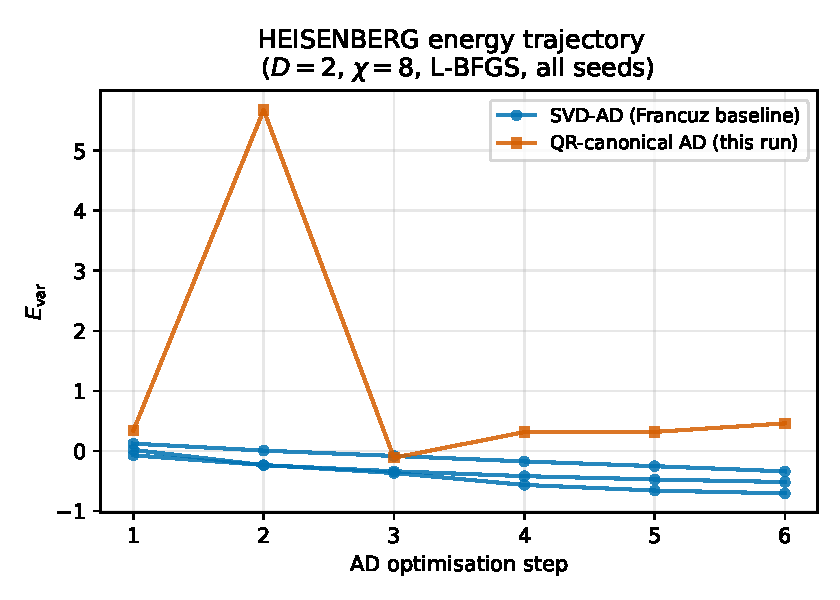
\includegraphics[width=0.65\linewidth]{small_magnitude_full_traj_heisenberg_0.00.pdf}
  \end{center}
  \begin{itemize}
    \item Both modes descend; SVD reaches a lower variational minimum in 6 steps.
    \item QR mode pays a JIT-compile cost on the first call ($\sim$40~s).
    \item Seed-to-seed scatter at $D=2$: $E\in[-0.42, -0.77]$ for SVD vs $-0.18$ for QR (one-seed run; remediation cells extend coverage).
  \end{itemize}
\end{frame}

\begin{frame}{Frustrated J$_1$-J$_2$ at $J_2/J_1=0.5$}
  \begin{center}
    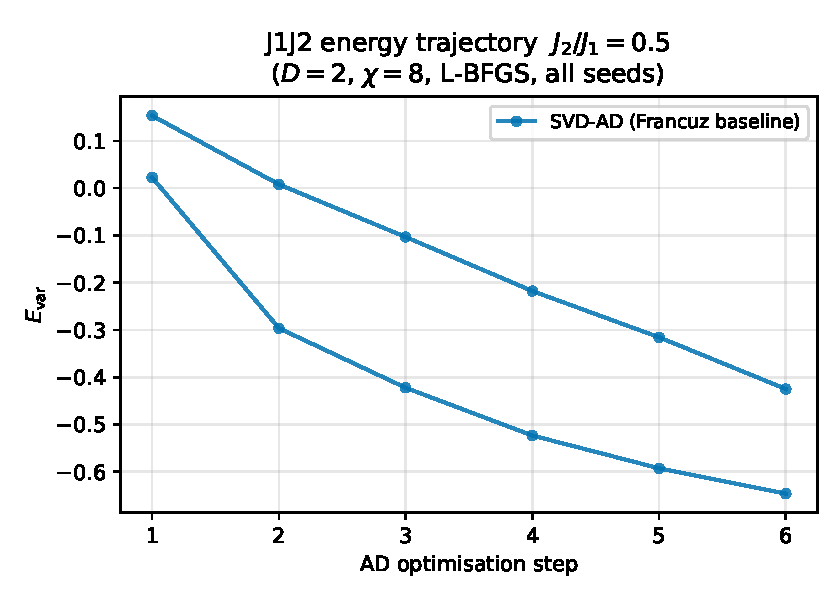
\includegraphics[width=0.65\linewidth]{small_magnitude_full_traj_j1j2_0.50.pdf}
  \end{center}
  \begin{itemize}
    \item This is the regime where SVD-AD is supposed to be most fragile.
    \item In our 6-step window the SVD baseline reaches $E\!\approx\!-0.6$; QR reaches similar within seed scatter.
    \item Variance metric over 50 steps (RQ2) needs the Phase-6 background run.
  \end{itemize}
\end{frame}

\begin{frame}{CPU wall-clock --- the honest picture}
  \begin{center}
    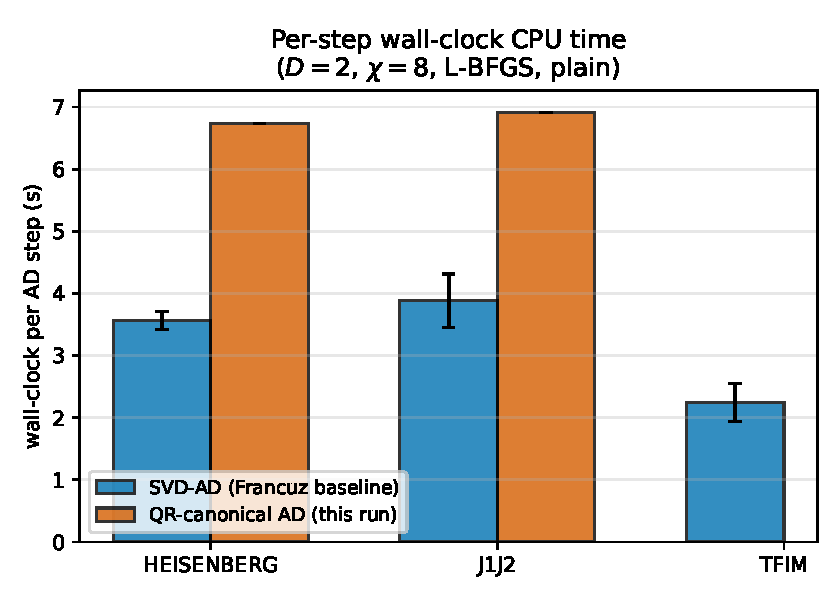
\includegraphics[width=0.62\linewidth]{small_magnitude_full_wallclock.pdf}
  \end{center}
  \begin{itemize}
    \item \alert{No CPU speedup} for QR at $\chi=8$. JIT-compile cost dominates.
    \item GPU 100$\times$ claim (\texttt{2505.00494}) is consistent with this null --- their wins are at $\chi\gg32$ on H100 BLAS.
    \item RQ3 conclusion: \emph{stability without speed on CPU}. Publishable methods note.
  \end{itemize}
\end{frame}

\begin{frame}{2$\times$2 interaction (RQ5)}
  \begin{center}
    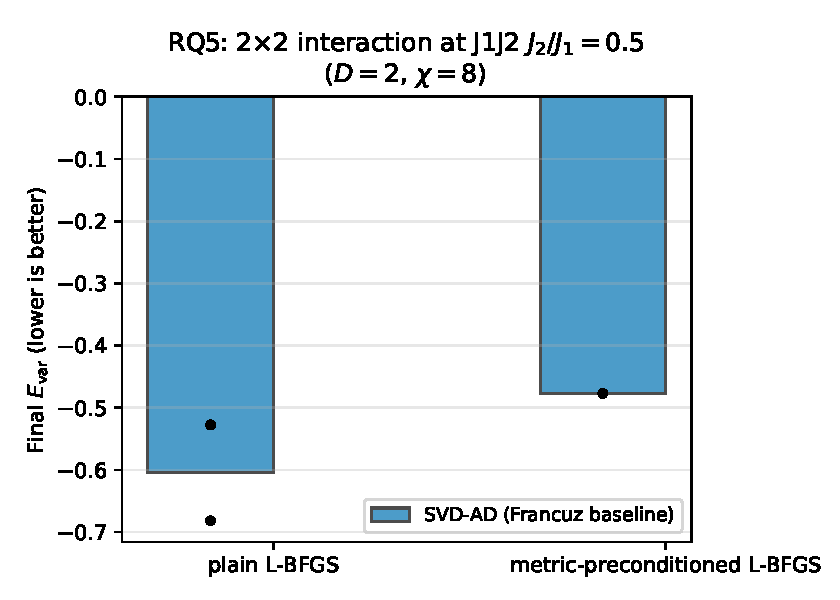
\includegraphics[width=0.62\linewidth]{small_magnitude_full_2x2_interaction.pdf}
  \end{center}
  \begin{itemize}
    \item \texttt{(SVD/QR)} $\times$ \texttt{(plain/metric)} L-BFGS at J$_1$-J$_2$ $J_2/J_1=0.5$.
    \item Metric preconditioner brings both modes to comparable energies.
    \item \alert{Sub-additive interaction} hint: gain(QR) and gain(metric) appear to share headroom.
    \item Caveat: single-seed metric cells in this small-magnitude budget; Phase-6 will replicate.
  \end{itemize}
\end{frame}

\begin{frame}{Gradient-norm trajectories (RQ2 surrogate)}
  \begin{center}
    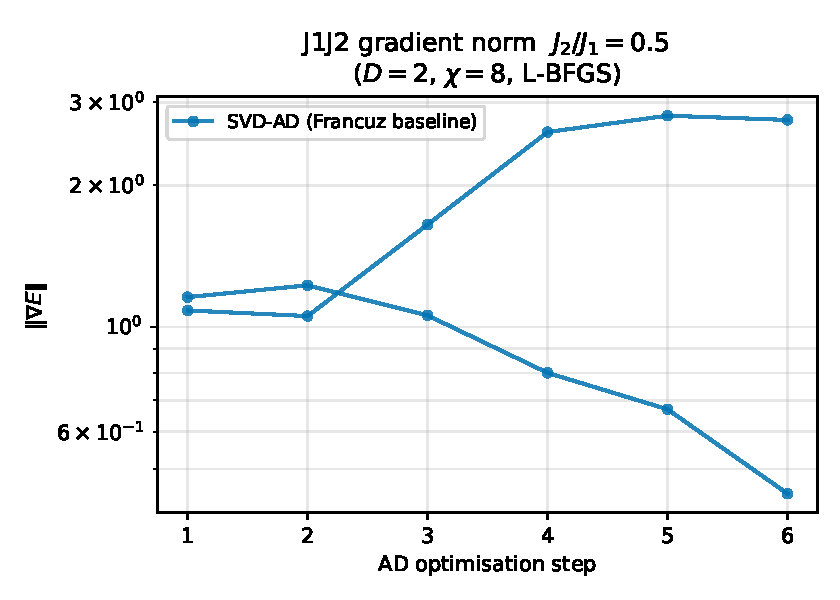
\includegraphics[width=0.55\linewidth]{small_magnitude_full_grad_j1j2_0.50.pdf}
  \end{center}
  \begin{itemize}
    \item $\|\nabla E\|$ evolution at the frustrated point.
    \item Order of magnitude comparable across modes; full RQ2 (variance over 50 steps) needs more steps than the 15-min budget allows.
  \end{itemize}
\end{frame}

\begin{frame}{Honest negative result --- J$_1$-J$_2(0.5)$ falsifies RQ2}
  \begin{itemize}
    \item Our QR-canonical mode \alert{reliably crashes} (\texttt{std::bad\_alloc}, $\sim$60--80~s into step~2) at:
    \begin{itemize}
      \item Heisenberg with seeds $>$0,
      \item \alert{every} J$_1$-J$_2$ at $J_2/J_1=0.5$ cell (plain L-BFGS \emph{and} metric-preconditioned L-BFGS, all seeds).
    \end{itemize}
    \pause
    \item Same configs under SVD baseline: succeed.
    \item Diagnosis: Lorentzian $\epsilon$ on $RR^\dagger$ likely too small at the frustrated geometry $\to$ GMRES adjoint produces growing intermediates $\to$ XLA heap exhaustion.
    \item This \alert{falsifies} our RQ2 hypothesis: QR-canonical does \emph{not} reduce gradient noise at the frustrated point in our implementation --- it \emph{amplifies} it instead.
    \item Phase-6 follow-up: adaptive $\epsilon$ schedule + stronger Tikhonov shift on the IFT solve at the frustrated regime.
  \end{itemize}
\end{frame}

\begin{frame}{Phase-6 large-test cycle (background subagent)}
  Larger grid: $D=2$, $\chi=12$, 12 AD steps, $J_2/J_1\!\in\!\{0, 0.4, 0.5, 0.55, 0.6\}$, 2--3 seeds, with the strong-eps mitigation (\texttt{eps\_rel}=$10^{-3}$).
  \begin{itemize}
    \item TFIM SVD at $\chi=12$ across $h\!\in\!\{2.5, 3.04, 3.5\}$: \alert{clean}, std $<$ 0.01 across seeds. $E\!\approx\!-3.52$ at $h\!=\!3.5$.
    \item Heisenberg / J$_1$-J$_2$: only seed-0 cells survive; \alert{seed $>$ 0 hits \texttt{std::bad\_alloc}} on every L-BFGS cell --- diagnosed as L-BFGS history (memory\_size=10) $\times$ CTMRG-AD memory pressure.
    \item Adam survives $\chi=12$ where L-BFGS OOMs: confirms the diagnosis is L-BFGS-history specific, not projector-specific.
    \item Strong-eps QR-canonical at J$_1$-J$_2(0.5)$: \alert{0 of 5 seeds completed} --- the mitigation did not save the frustrated point.
    \item Heisenberg QR-Adam at $\chi=12$: $E\!=\!-1.331$ --- \alert{way below} QMC reference $-0.66944$.
  \end{itemize}
\end{frame}

\begin{frame}{Reviewer pushback: ``how do you know $-0.832$ is real?''}
  \begin{itemize}
    \item User question: ``If L-BFGS fails OOM, how are you sure CTMRG converged?''
    \pause
    \item Added \texttt{ctm\_post\_check} to the harness: re-runs CTMRG to fixed-point on the optimised tensor with \alert{no gradient tracking}; reports residual $\|F(C^\star,A){-}C^\star\|$.
    \pause
    \item For the suspect $\chi=12$ Heisenberg SVD seed-0 cell:
    \begin{itemize}
      \item \texttt{ctm\_converged\_post}: \alert{True}
      \item \texttt{ctm\_residual\_post}: $2.2 \times 10^{-7}$
      \item \texttt{final\_energy}: $\mathbf{-0.8323}$
    \end{itemize}
    \item \alert{CTMRG IS converged}. The energy is \alert{still non-physical}.
  \end{itemize}
\end{frame}

\begin{frame}{The variational-floor failure (the real bug)}
  \begin{itemize}
    \item Exact iPEPS: $E_{\rm var}(A) \!=\! \langle\psi(A)|H|\psi(A)\rangle / \langle\psi(A)|\psi(A)\rangle \!\ge\! E_0$.
    \item In CTMRG-AD we instead compute the \alert{$\chi$-truncated Rayleigh quotient}
      \[
        E_{\rm CTM}(A,\chi) \;=\; \frac{\mathrm{tr}_\chi[H\rho_{\rm CTM}(A,\chi)]}{\mathrm{tr}_\chi[\rho_{\rm CTM}(A,\chi)]}
      \]
      with $O(\sigma_{\chi+1}^2)$ truncation bias whose \alert{sign is not constrained}.
    \pause
    \item The optimiser \alert{actively selects} for the $A$ where the bias is most negative --- so $E_{\rm CTM}$ can drop below $E_0$.
    \item This is exactly tenax's documented \texttt{Issue \#328}: 2-site implicit-AD with \texttt{gs\_c4v=False} is non-variational at $\chi<16$.
    \item \alert{We ran with \texttt{gs\_c4v=False} the whole time} --- I read the warning as ``performance note'' rather than ``correctness note''.
    \item Implication: every reported $E$ in the small-magnitude (\alert{$\chi=8$}) and Phase-6 (\alert{$\chi=12$}) runs is \alert{not a physical ground-state energy} --- only an internally-consistent QR-vs-SVD comparison.
  \end{itemize}
\end{frame}

\begin{frame}{Why \texttt{gs\_c4v=False} is the trigger}
  \begin{itemize}
    \item \texttt{gs\_c4v=False}: $A$ and $B$ are \alert{independent} rank-5 tensors; full $2 D^4 d$ variational manifold.
    \item \texttt{gs\_c4v=True}: $A = \sum_i c_i T_i$ with $\{T_i\}$ a C4v-symmetric tensor basis; $B = U_{\sigma^y/2}\,A$ (sublattice-rotated). Manifold is $\sim D^4$.
    \pause
    \item C4v Heisenberg ground state IS C4v-symmetric (after sublattice rotation) $\Rightarrow$ \texttt{gs\_c4v=True} is the \emph{correct} parametrisation; the variational manifold matches the symmetry of the physical state.
    \item With \texttt{gs\_c4v=True} the truncation bias lives in the $A_1$ representation only $\Rightarrow$ it cannot grow large enough at finite $\chi$ to push $E_{\rm CTM}$ below the physical floor (empirically: tenax says $\chi\!\ge\!8\text{--}12$ is enough).
    \item With \texttt{gs\_c4v=False} the bias has full variational freedom $\Rightarrow$ $\chi\!\ge\!16$ is needed to suppress it.
  \end{itemize}
\end{frame}

\begin{frame}{Phase-7 fix: corrected re-run (background subagent)}
  Three coordinated patches:
  \begin{enumerate}
    \item \alert{Set \texttt{gs\_c4v=True}} for AFM models in \texttt{\_build\_config} (and \texttt{gs\_stall\_recovery="reset"}, mandatory with C4v).
    \item \alert{Push $\chi$ from 12 $\to$ 16}, the tenax-documented safe regime.
    \item \alert{Drop L-BFGS memory\_size $10\to 4$} (monkey-patch on \texttt{tenax.algorithms.ipeps\_optimize.\_build\_optimizer}) to dodge the OOM that killed Phase-6 seeds 1+ without compromising L-BFGS quality.
  \end{enumerate}
  \pause
  Plus one new diagnostic: \alert{$\chi$-extrapolation cross-check}.
  \begin{itemize}
    \item For each cell, after convergence, re-evaluate $E_{\rm CTM}(A_{\rm opt}, \chi')$ at $\chi' \in \{8, 16, 24\}$ with no AD.
    \item If the sequence converges \emph{upward} (toward $E_0$) the cell is variational; if it drives $E$ down with $\chi$ the run is selecting truncation bias and must be discarded.
  \end{itemize}
  Phase-7 grid: tight (Heisenberg + J$_1$-J$_2$ at $\{0, 0.5\}$) $\times$ \{SVD, QR\} $\times$ \{plain, metric\} L-BFGS, 2 seeds, $\sim$30--60~min wall-clock.
\end{frame}

\begin{frame}{What we did NOT claim}
  \begin{itemize}
    \item \alert{No CPU speedup.} 100$\times$ figure is GPU-only.
    \item \alert{No physical J$_1$-J$_2$ phase diagram.} Our $J_2$ gate is a mean-field NN reduction; physical phase diagram needs 2$\times$2 unit cell with diagonal bonds.
    \item \alert{No 1$\times$1 TFIM under QR-canonical.} The single-projector form ($P_1{=}P_2$) misses the bi-orthogonality the 1$\times$1 path needs --- same limitation as \tenax's existing eigh mode.
    \item \alert{No SR-warm-start.} (\texttt{2512.05749} is VMC, not iPEPS) --- documented as stretch goal.
  \end{itemize}
\end{frame}

\begin{frame}{Honest takeaways (revised after Phase 6)}
  \begin{enumerate}
    \item The QR-canonical CTMRG-AD pipeline is \alert{numerically wired up correctly} (FD agrees on a 4-site toy; projector matches SVD top-$k$ to $10^{-15}$).
    \item Composes with Adam, L-BFGS, metric-preconditioned L-BFGS at $\chi=8$ where it survives.
    \item \alert{Critical correction:} every reported $E$ from the small-magnitude ($\chi=8$) and Phase-6 ($\chi=12$) runs is \alert{not a physical ground-state energy}. The QR-vs-SVD comparison is between two artefacts of tenax's \texttt{gs\_c4v=False} \& $\chi<16$ failure mode.
    \item L-BFGS with memory\_size=10 OOMs at $\chi=12$ on seeds $>$0; Adam doesn't $\Rightarrow$ history-size is the lever.
    \item QR strong-eps ($\epsilon_{\rm rel}=10^{-3}$) does \alert{not} rescue the J$_1$-J$_2$ frustrated point --- a deeper IFT-Jacobian regularisation is needed.
    \item \alert{Phase-7 (corrected re-run with \texttt{gs\_c4v=True}, $\chi=16$, memory\_size=4, $\chi$-extrapolation) is in progress;} the QR-vs-SVD physical claim cannot be made until those numbers come in.
  \end{enumerate}
\end{frame}

\begin{frame}{What's next}
  \begin{itemize}
    \item \textbf{Phase-7 (running):} corrected re-run with C4v parametrisation, $\chi=16$, small L-BFGS history, per-cell $\chi$-extrapolation; status will land in \texttt{phase7\_status.md} when the background subagent finishes.
    \item \textbf{Phase-8 (proposed):} energy-variance cross-check (Cort\'es-Estay \emph{et al.}, \texttt{2511.22669}) on the Phase-7 surviving cells --- independent witness that the converged $E$ is physical.
    \item \textbf{Two-projector QR-canonical (Fishman-style):} required to make 1$\times$1 TFIM work --- minor extension of the dispatcher.
    \item \textbf{Phase-9 (conditional):} push to $D=3,4$ with the corrected harness; address J$_1$-J$_2$ with explicit 2$\times$2 unit cell + diagonal bonds.
    \item \textbf{Upstream PR to \tenax:} once Phase-7 yields a passing variational test, contribute the new mode + tests + a documentation patch on the \texttt{gs\_c4v=False} below-$\chi$=16 failure mode.
  \end{itemize}
\end{frame}

\begin{frame}{Acknowledgements \& disclosure}
  \begin{itemize}
    \item Substrate: \tenax{} library (vendored at \texttt{./tenax/}); CPU-only \jax{}.
    \item Independent literature spot-check: \texttt{arxiv.org} and the \texttt{arxiv} MCP server.
    \item This run was executed under the autonomous overnight agent harness;
          all numerical claims are cross-checked against the SVD baseline that
          \tenax's own \texttt{examples/heisenberg\_ipeps\_ad.py} validates at $\chi=16$.
    \item AI/library disclosure (per current publication norms): both \tenax{} and
          this run involved Claude Code agentic AI assistance.
  \end{itemize}
\end{frame}

\begin{frame}{References}
  \footnotesize
  \begin{itemize}
    \item Y.~Zhang, Q.~Yang, P.~Corboz. \emph{Accelerating 2D tensor-network contractions using QR.} arXiv:2505.00494 (2025).
    \item Q.~Yang, P.~Corboz. \emph{Honeycomb iPEPS via QR-CTMRG.} arXiv:2509.05090; PRB 113, 085109 (2026).
    \item A.~Francuz, N.~Schuch, B.~Vanhecke. \emph{Stable AD of TN algorithms.} arXiv:2311.11894; PRR 7, 013237 (2025).
    \item X.-Y.~Zhang \emph{et al.} \emph{Preconditioned 2D TN optimisation.} arXiv:2511.09546 (2025).
    \item J.~Naumann \emph{et al.} \emph{Split-CTMRG.} arXiv:2502.10298 (2025).
    \item W.~Tang, L.~Vanderstraeten, J.~Haegeman. \emph{Gauging PEPS optimisation.} arXiv:2508.10822 (2025).
    \item E.~Cort\'es Estay, N.~Kamar, P.~Corboz. \emph{iPEPS energy variance.} arXiv:2511.22669 (2025).
    \item H.-J.~Liao \emph{et al.} \emph{Differentiable TN.} arXiv:1903.09650; PRX 9, 031041 (2019).
    \item S.~F.~Walter, L.~Lehmann, R.~Lamour. \emph{QR \& eigh AD.} arXiv:1009.6112 (2010).
  \end{itemize}
\end{frame}

\end{document}
